\documentclass[parskip=full]{scrartcl}
\usepackage[utf8]{inputenc} % use utf8 file encoding for TeX sources 

\usepackage[T1]{fontenc} % avoid garbled Unicode text in pdf 
\usepackage[german]{babel} % german hyphenation, quotes, etc 
\usepackage{hyperref} % detailed hyperlink/pdf configuration
\usepackage{graphicx}
\usepackage[toc]{glossaries}
\usepackage{caption}
\usepackage{pdfpages}
\hypersetup{ % ‘texdoc hyperref‘ for options 
	pdftitle={Entwurf}, %
	bookmarks=true,%
}
\usepackage{csquotes} % provides \enquote{} macro for "quotes"
\usepackage{enumitem}
\makeglossaries



\newglossaryentry{FCM}
{
	name={FCM},
	description={Firebase Cloud Messaging \href{https://firebase.google.com/docs/cloud-messaging/}{https://firebase.google.com/docs/cloud-messaging/}},
	first={Firebase Cloud Messaging(FCM)},
	long={Firebase Cloud Messaging}
}
\begin{document}
	\begin{titlepage}
			
		\centering
		\vspace*{0.2\textheight}
		{\Large Praxis der Softwareentwicklung}\\[\baselineskip]
		\vspace{2cm}
		{\Huge \textbf{Entwurf der Schach-App}}\\[\baselineskip]\par
		\vspace{2cm}
		{\LARGE Rukiye Devran, Tim Groß, Daniel Helmig, Orkhan Aliev}\par		
		\newpage	
		\tableofcontents
		\pagebreak
		
	\end{titlepage}
	\section{Einleitung}
		bli bla blub
	\section{Klassendiagramme}
	
		\subsection{Spiel}
		
		\begin{minipage}{\linewidth}
			\centering
			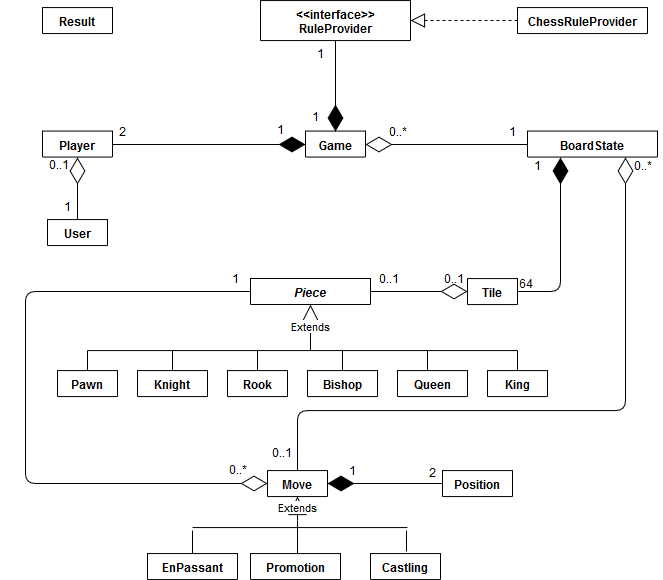
\includegraphics[width=1\linewidth]{Diagramme/TotalGame}
			\captionof{figure}{TotalGame}
			\label{fig:totalGame}
		\end{minipage}
		\newpage
		\begin{itemize}
			\item \textbf{\textit{Spiel}}
				\begin{description}
					\item \textbf{\textit{Game}} stellt ein Spiel dar. Es besteht aus zwei Spielern \textbf{\textit{Player}} und einem Spielfeld \textbf{\textit{BoardState}}. Außerdem benutzt es eine Instanziierung des Interface \textbf{\textit{RuleProvider}}.
					\item In diesem Fall wird das Interface nur von \textbf{\textit{ChessRuleProvider}} implementiert. Dieser benutzt als Rückgabewert einer Methode die Klasse \textbf{\textit{Result}}.
					\item Ein \textbf{\textit{Player}} besteht aus einem \textbf{\textit{User}}. Umgekehrt muss ein \textbf{\textit{User}} aber nicht zu jedem Zeitpunkt einen \textbf{\textit{Player}} haben.
					\item \textbf{\textit{BoardState}} enthält 64 \textbf{\textit{Tiles}} und einen \textbf{\textit{Move}}, welcher hier den letzten ausgeführten Zug darstellt. 
					\item Ein \textbf{\textit{Tile}} kann ein \textbf{\textit{Piece}} enthalten, muss es aber nicht.
					\item \textbf{\textit{Piece}} ist eine abstrakte Klasse und stellt eine Figur dar. Sie wird von den sechs konkreten Figurenklassen beerbt.
					\item Ein \textbf{\textit{Move}} besteht im Allgemeinen nur aus zwei \textbf{\textit{Positionen}}. Es gibt drei Spezialfälle eines Zuges, welche eine gesonderte Implementierung benötigen, da sie aus mehr als nur zwei \textbf{\textit{Positionen}} bestehen.
					\item \textbf{\textit{Position}} Stellt eine Position auf einem Schachbrett dar und besteht aus zwei Zahlen, welche die Koordinaten darstellen.
				\end{description}
		
		\end{itemize}
		\newpage
		
		\subsubsection{Game}
		\begin{minipage}{\linewidth}
			\centering
			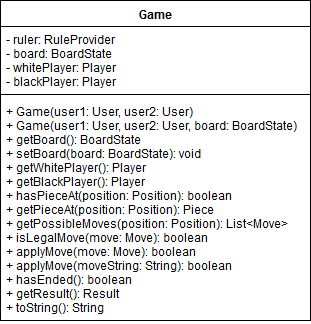
\includegraphics[width=1\linewidth]{Diagramme/Game}
			\captionof{figure}{Game}
			\label{fig:game}
		\end{minipage}
		\begin{itemize}
			\item \textbf{Game}
			
			Stellt ein Spiel dar, verwaltet teilnehmende Spieler, Regelwerk sowie Brettzustand
				
				Attribute
				\newline
				\rule{\textwidth}{1pt}
				
				\begin{description}
					 \item \textbf{\textit{ruler:}} Objekt, welches die Spielregeln zur Verfügung stellt.
					 \item \textbf{\textit{board:}} Hier wird der aktuelle Spielstatus gespeichert.
					 \item \textbf{\textit{whitePlayer:}} Der Spieler mit den weißen Figuren.
					 \item \textbf{\textit{blackPlayer:}} Der Spieler mit den schwarzen Figuren.
				\end{description}
				 Methoden
				 \newline
		 		\rule{\textwidth}{1pt}
	 			\begin{description}
					 \item \textbf{\textit{Game(User user1, User user2)}} Konstruktor, welcher ein Spiel mit den Standard Schachregeln und einem Brett auf Anfangsposition erzeugt. Der zuerst übergebene User erhält die weißen Figuren, der zweite die schwarzen.
					 \item \textbf{\textit{Game(User user1, User user2, BoardState board)}} Konstruktor, welcher ein Spiel mit den Standard Schachregeln und dem übergebenen Brettstatus erzeugt. Der zuerst übergebene User erhält die weißen Figuren, der zweite die schwarzen.
					 \item \textbf{\textit{getBoard():}} Gibt den Brettstatus des akutellen Spiels als Objekt zurück.
					\item \textbf{\textit{getBoard(BoardState board):}} Setzt den Brettstatus auf das übergebene Objekt.
					\item \textbf{\textit{getWhitePlayer():}} Gibt den weißen Spieler zurück.
					\item \textbf{\textit{getBlackPlayer():}} Gibt den schwarzen Spieler zurück.
					\item \textbf{\textit{hasPieceAt(Position position):}} Gibt zurück, ob sich an der übergebenen Position auf dem Brett eine Figur befindet.
					\item \textbf{\textit{getPieceAt(Position position):}} Gibt die Figur zurück, welche sich an der übergebenen Position befindet. Ist die Position nicht besetzt, wird null zurückgegeben.
					\item \textbf{\textit{getPossiblePositions(Position position):}} Gibt alle möglichen Positionen als Liste zurück, auf welche eine Figur, welche sich auf der übergebenen Position befindet, ziehen kann. Zum Berechnen dieser wird das \textbf{\textit{ruler}} Objekt benutzt.
					\item \textbf{\textit{applyMove(Move):}} Führt einen übergebenen Zug auf dem Brett aus.
					\item \textbf{\textit{applyMove(String):}}Führt einen als String übergebenen Zug auf dem Brett aus. Dazu muss der String erst in ein Zugobjekt umgewandelt werden.
					\item \textbf{\textit{hasEnded():}} Gibt zurück, ob das Spiel gemäß den Schachregeln beendet ist. Dazu wird das \textbf{\textit{ruler}} Objekt benutzt.
					\item \textbf{\textit{getResult():}} Gibt das Ergebnis eines Spiels zurück. Ist das Spiel noch nicht beendet, wird null zurückgegeben.
					\item \textbf{\textit{toString():}} Wandelt den gesamten Spielstatus in eine Zeichenkette um. Dazu werden die Benutzernamen sowie die String-Repräsentation des \textbf{\textit{board}} Objekts genutzt.
				\end{description}
			
		\end{itemize}		
		\newpage
		
		\subsubsection{RuleProvider}
		\begin{minipage}{\linewidth}
			\centering
			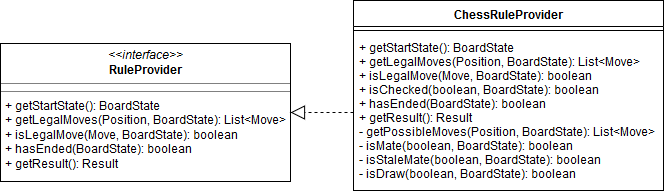
\includegraphics[width=1\linewidth]{Diagramme/RuleProvider}
			\captionof{figure}{RuleProvider}
			\label{fig:ruleProvider}
		\end{minipage}
		\begin{itemize}
			\item \textbf{RuleProvider}
			
			Interface, welches alle nötigen Regeln eines Spiels auf einem Schachbrett bereitstellt. Die zu implementierenden Methoden sind:
			
				Methoden
				\newline
				\rule{\textwidth}{1pt}
				\begin{description}			
					\item \textbf{\textit{getStartState():}} Soll die Anfangskonfiguration eines Brettes für das jeweilige Spiel zurückgeben.
					\item \textbf{\textit{getLegalMoves(Position position, BoardState board):}} Soll auf einem Brett ausgehend von einer Position die Zugmöglichkeiten der sich darauf befindenden Figur berechnen, entsprechend der implementierten Regeln.
					\item \textbf{\textit{isLegalMove(Move move, BoardState board):}} Soll überprüfen, ob ein Zug gemäß der jeweiligen Regeln auf einem bestimmten Brett erlaubt ist.
					\item \textbf{\textit{hasEnded(BoardState board):}} Soll prüfen, ob das Spiel auf einem bestimmten Brett gemäß den jeweiligen Regeln beendet ist.
					\item \textbf{\textit{getResult(BoardState board):}} Soll das Ergebnis eines Spiels zurückgeben. Ist das Spiel nicht beendet soll null zurückgegeben werden.
				\end{description}
			
			\item \textbf{ChessRuleProvider}
			
			Konkreter Regellieferer, welcher die genauen Schachregeln zur Verfügung stellt.
			
				Methoden
				\newline
				\rule{\textwidth}{1pt}
				\begin{description}
					\item \textbf{\textit{getStartState():}} Gibt die Standard Anfangsstellung eines Schachspiels als \textbf{\textit{BoardState}} zurück.
					\item \textbf{\textit{getLegalMoves(Position position, BoardState board):}} Gibt eine Liste an erlaubten Zügen ausgehend von einer ausgewählten Position und einem Brett zurück. Dazu werden zunächst mit \textbf{\textit{getPossibleMoves(Position, BoardState)}} alle möglichen Züge berechnet. Anschließen wird jeder Zug auf einer Kopie des Brettes simuliert, und mithilfe von \textbf{\textit{isChecked(boolean, BoardState)}} überprüft, ob der selbe Spieler danach im Schach stünde (was den Zug ungültig machen würde).
					\item \textbf{\textit{isLegalMove(Move move, BoardState board):}} Prüft, ob ein Zug gemäß den Schachregeln auf dem übergebenen Brett erlaubt ist.
					\item \textbf{\textit{isChecked(boolean white, BoardState board):}} Überprüft ob ein Spieler auf dem gegebenen Brett im Schach steht. Ist der übergebene boolean true, wird Weiß überprüft, bei false Schwarz. Dazu wird geschaut, ob es eine gegnerische Figur gibt, welche durch \textbf{\textit{getPosssibleMoves(Position position, BoardState board)}} einen Zug erhält, mit welchem der gegnerische König erreicht werden könnte.
					\item \textbf{\textit{hasEnded(BoardState board):}} Prüft, ob das Schachspiel zu Ende ist. Dazu wird geprüft, ob der zu ziehende Spieler laut \textbf{\textit{isMate(BoardState board)}} Matt gesetzt, laut \textbf{\textit{isStaleMate(BoardState board)}} Patt gesetzt oder ob laut  \textbf{\textit{isDraw(BoardState board)}} andersweitig ein Unentschieden erreicht wurde.
					\item \textbf{\textit{getResult()}} Ruft \textbf{\textit{hasEnded(BoardState board)}} auf, gibt aber bei beendetem Spiel das jeweilige Ergebnis als Result mit Begründung zurück. Ist das Spiel nicht beendet wird null zurückgegeben.
					\item \textbf{\textit{getPossibleMoves(Position position, BoardState board):}} Gibt alle möglichen Züge einer Figur auf dem Brett zurück, ohne dabei zu berücksichtigen, ob der ziehende Spieler nach diesem Zug im Schach stehen würde. Dazu wird die jeweilige getMovement()-Methode der Figur an der angegebenen Position ausgeführt.				
					\item \textbf{\textit{isMate(BoardState board):}} Prüft, ob der zu ziehende Spieler Matt gesetzt wurde. Das ist der Fall, wenn der Spieler laut \textbf{\textit{isChecked(boolean, BoardState)}} im Schach steht, und es für keine Figur einen nach \textbf{\textit{getLegalMoves(Position, BoardState)}}erlaubten Zug gibt.
					\item \textbf{\textit{isStaleMate(BoardState board):}} Prüft, ob der zu ziehende Spieler Patt gesetzt wurde. Das ist der Fall, wenn der Spieler laut \textbf{\textit{isChecked(boolean, BoardState)}} nicht im Schach steht, und es für keine Figur einen nach \textbf{\textit{getLegalMoves(Position, BoardState)}}erlaubten Zug gibt.
					\item \textbf{\textit{isDraw(BoardState board):}} Prüft, ob ein anderweitiges Unentschieden erreicht wurde. Dies ist der Fall, wenn zu wenig Figuren auf dem Brett vorhanden sind um Matt zu setzen, oder wenn 50 Züge lang keine Figur geschlagen und kein Bauer gezogen wurde.
				\end{description}
		\end{itemize}
		\newpage
		\subsubsection{BoardState}
		\begin{minipage}{\linewidth}
			\centering
			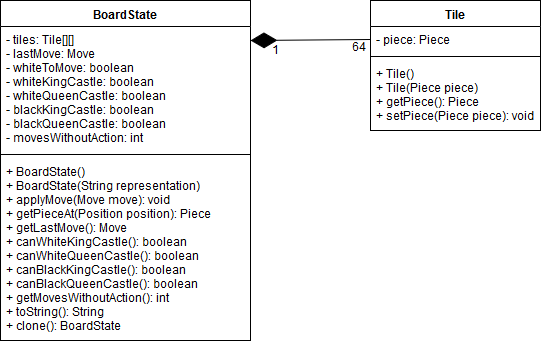
\includegraphics[width=1\linewidth]{Diagramme/BoardState}
			\captionof{figure}{BoardState}
			\label{fig:boardState}
		\end{minipage}
	
		\begin{itemize}
			\item \textbf{\textit{BoardState}}	
			
			Der gesamte Status eines Schachspiels der notwendig ist, um ein Spiel rekonstriuren und alle Regeln überprüfen zu können.
			
				Attribute
				\newline
				\rule{\textwidth}{1pt}
			
				\begin{description}				
					\item \textbf{\textit{tiles:}} Ein Array von Tiles, welches den Aufbau des Spielbretts darstellt
					 \item \textbf{\textit{lastMove:}} Der letzte gespielte Zug.
					 \item \textbf{\textit{whiteToMove:}} Speichert, ob Weiß am Zug ist.
					 \item \textbf{\textit{whiteKingCastle:}} Speichert ab, ob Weiß noch auf der Königsseite rochieren kann.
					 \item \textbf{\textit{whiteQueenCastle:}} Speichert ab, ob Weiß noch auf der Damenseite rochieren kann.
					 \item \textbf{\textit{blackKingCastle:}} Speichert ab, ob Schwarz noch auf der Königsseite rochieren kann.
					 \item \textbf{\textit{blackQueenCastle:}} Speichert ab, ob Schwarz noch auf der Damenseite rochieren kann.
					\item \textbf{\textit{movesWithoutAction:}} Speichert die Anzahl der Züge in Folge, in welcher kein Bauer gezogen und keine Figur geschlagen wurde.
				\end{description}
				Methoden
				\newline
				\rule{\textwidth}{1pt}
				\begin{description}
					\item \textbf{\textit{BoardState():}} Erzeugt ein leeres Schachbrett und setzt alle Variablen auf ihre Standardwerte.
					\item \textbf{\textit{BoardState(String representation):}} Erzeugt ein Brett, ausgehen von einem String. In diesem müssen alle notwenidigen Informationen in einem bestimmten Format gespeichert sein.
					\item \textbf{\textit{applyMove(Move move):}} Führt einen Zug auf dem Brett aus, indem es die Figur(en) wie im Move-Objekt vorgegeben bewegt und möglicherweise andere Figuren schlägt(überschreibt). Außerdem wird die zu ziehende Farbe, der letzte Zug, sowie die Anzahl der Züge ohne Aktion aktualisiert. Bei entsprechender Verletzung werden möglich Rochaden auf false gesetzt.
					\item \textbf{\textit{getPieceAt(Position position):}} Gibt die Figur an der übergebenen Position zurück. Ist die Position nicht besetzt, wird null zurückgegeben.			
					\item \textbf{\textit{getLastMove():}} Gibt \textbf{\textit{lastMove}} zurück.
					 \item \textbf{\textit{canWhiteKingCastle():}} Gibt zurück, ob Weiß noch auf der Königsseite rochieren kann.
					 \item \textbf{\textit{canWhiteQueenCastle():}} Gibt zurück, ob Weiß noch auf der Damenseite rochieren kann.
					 \item \textbf{\textit{canBlackKingCastle():}} Gibt zurück, ob Schwarz noch auf der Königsseite rochieren kann.
					 \item \textbf{\textit{canBlackQueenCastle():}} Gibt zurück, ob Schwarz noch auf der Damenseite rochieren kann.
					 \item \textbf{\textit{getMovesWithoutAction):}} Gibt \textbf{\textit{movesWithoutAction}} zurück.
					 \item \textbf{\textit{toString()}} Gibt den gesamten Brettzustand als String codiert zurück. Aus diesem String muss mithilfe des entsprechenden Konstruktors ein identisches Brett erzeugt werden können.		
					 \item \textbf{\textit{clone():}} Erzeugt und übergibt ein identisches Spielbrett, indem die String-Repräsentation des aktuellen Brettes als Parameter des Konstruktors verwendet wird.				
				\end{description}
			
			\item \textbf{\textit{Tile}}
			
			Stellt eine Feld eines Schachbretts dar.
			
				Attribute
				\newline
				\rule{\textwidth}{1pt}
			
				\begin{description}					
					\item \textbf{\textit{piece}} Die Figur, welche sich auf dem Feld befindet. Befindet sich keine Figur auf dem Feld, steht hier null.
				\end{description}
				Methoden
				\newline
				\rule{\textwidth}{1pt}
				\begin{description}
					\item \textbf{\textit{Tile():}} Konstruktor, welcher ein leeres Feld erzeugt.
					\item \textbf{\textit{Tile(Piece):}} Konstruktor, welcher ein Feld mit der übergebenen Figur darauf erzeugt.
					\item \textbf{\textit{getPiece():}} Gibt \textbf{\textit{piece}} zurück.
					\item \textbf{\textit{setPiece(Piece piece):}} Setzt \textbf{\textit{piece}} auf die übergebene Figur.
				\end{description}
			
		\end{itemize}
		\newpage		
		
		\subsubsection{Player}
		\begin{minipage}{\linewidth}
			\centering
			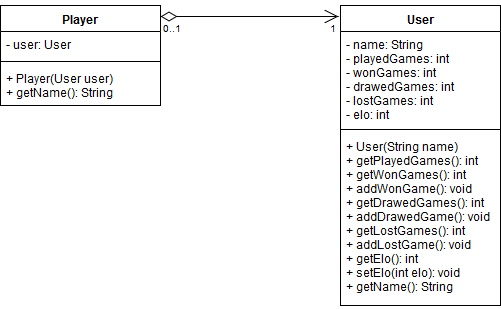
\includegraphics[width=1\linewidth]{Diagramme/Player}
			\captionof{figure}{Player}
			\label{fig:player}
		\end{minipage}
		\begin{itemize}
			\item \textbf{\textit{Player}}
			
			Stellt einen Spieler eines konkretes Spiels dar. Existiert nur während das jeweilige Spiel existiert.
			
				Attribute
				\newline
				\rule{\textwidth}{1pt}
				
				\begin{description}					
					\item \textbf{\textit{user:}} Der mit diesem Spielerobjekt verknüpfte Benutzer
				\end{description}
				Methoden
				\newline
				\rule{\textwidth}{1pt}
				\begin{description}
					\item \textbf{\textit{Player(User user):}} Konstruktor, welcher \textbf{\textit{user}} auf den übergebenen User setzt.
					\item \textbf{\textit{getName():}} Gibt den Namen des verknüften Benutzers als String zurück.
				\end{description}
			
			\item \textbf{\textit{User}}
			
				Attribute
				\newline
				\rule{\textwidth}{1pt}
				
				\begin{description}
					\item \textbf{\textit{name:}} Der eindeutige Name eines Benutzers.
					\item \textbf{\textit{playedGames:}} Die Anzahl der gespielten Spiele des Benuters.
					\item \textbf{\textit{wonGames:}} Die Anzahl der gewonnenen Spiele des Benuters.
					\item \textbf{\textit{drawedGames:}} Die Anzahl der remisierten Spiele des Benuters.
					\item \textbf{\textit{lostGames:}} Die Anzahl der verlorenen Spiele des Benuters.
					\item \textbf{\textit{elo:}} Der Elo-Wert des Benutzers.
				\end{description}
				Methoden
				\newline
				\rule{\textwidth}{1pt}
				\begin{description}
					\item \textbf{\textit{User(String name):}} Erstellt einen neuen Benutzer mit dem übergebenen Namen. Setzt alle Attribute auf 0, \textbf{\textit{elo}} auf 1000.
					\item \textbf{\textit{getPlayedGames():}} Gibt \textbf{\textit{playedGames}} zurück.
					\item \textbf{\textit{getWonGames():}} Gibt \textbf{\textit{wonGames}} zurück.
					\item \textbf{\textit{addWonGame():}} Erhöht \textbf{\textit{wonGames}} und \textbf{\textit{playedGames}} um eins.
					\item \textbf{\textit{getDrawedGames():}} Gibt \textbf{\textit{drawedGames}} zurück.
					\item \textbf{\textit{addDrawedGame():}} Erhöht \textbf{\textit{drawedGames}} und \textbf{\textit{playedGames}} um eins.
					\item \textbf{\textit{getLostGames():}} Gibt \textbf{\textit{lostGames}} zurück.				
					\item \textbf{\textit{addLostGame():}} Erhöht \textbf{\textit{lostGames}} und \textbf{\textit{playedGames}} um eins.
					\item \textbf{\textit{getElo():}} Gibt \textbf{\textit{elo}} zurück.
					\item \textbf{\textit{setElo(int Elo):}} Setzt die Elo des Benutzers auf den übergebenen Wert.
					\item \textbf{\textit{getName():}} Gibt \textbf{\textit{name}} zurück.					
				\end{description}
		\end{itemize}
		\newpage	
			
		\subsubsection{Result}
		
		\begin{minipage}{\linewidth}
			\centering
			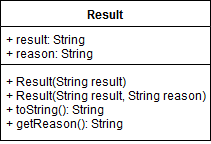
\includegraphics[width=1\linewidth]{Diagramme/Result}
			\captionof{figure}{Result}
			\label{fig:result}
		\end{minipage}
		\begin{itemize}
			\item \textbf{\textit{Result}}
			
			Stellt ein Ergebnis eines Spiels dar.
			
				Attribute
				\newline
				\rule{\textwidth}{1pt}
			
				\begin{description}					
					\item \textbf{\textit{result:}} Das Ergebnis eines Spiels als String codiert.
					\item \textbf{\textit{reason:}} Eine Begründung zum Ergebnis als String.
				\end{description}
				Methoden
				\newline
				\rule{\textwidth}{1pt}
				\begin{description}
					\item \textbf{\textit{Result(String result):}} Erzeugt ein Objekt mit dem übergebenen String als \textbf{\textit{result}} und einer leeren \textbf{\textit{reason}}.
					\item \textbf{\textit{Result(String result, String reason):}} Erzeugt ein Objekt mit dem ersten übergebenen String als \textbf{\textit{result}} und dem zweiten übergebenen String als \textbf{\textit{reason}}.
					\item \textbf{\textit{toString():}} Gibt \textbf{\textit{result}} zurück.
					\item \textbf{\textit{getReson():}} Gibt \textbf{\textit{reason}} zurück.						
				\end{description}
			
		\end{itemize}
		\newpage
		
		\subsubsection{Move}
		
		\begin{minipage}{\linewidth}
			\centering
			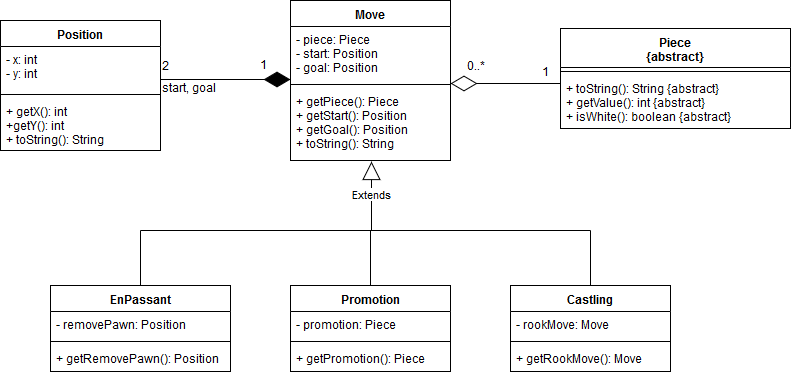
\includegraphics[width=1\linewidth]{Diagramme/Move}
			\captionof{figure}{Move}
			\label{fig:move}
		\end{minipage}
		\begin{itemize}
			\item \textbf{\textit{Move}}
			
			Stellt einen Zug dar, ohne über die zu ziehende Figur bescheid zu wissen.
			
				Attribute
				\newline
				\rule{\textwidth}{1pt}
			
				\begin{description}				
					\item \textbf{\textit{start:}} Position, von welcher aus der Zug ausgeführt wird.
					\item \textbf{\textit{goal:}} Position, zu welcher der Zug hinführt.
				\end{description}
				Methoden
				\newline
				\rule{\textwidth}{1pt}
				\begin{description}
					\item \textbf{\textit{Move(start: Position, goal: Position):}} Erzeugt einen Zug mit der übergebenen Start- und Zielposition.				
					\item \textbf{\textit{getStart():}} Gibt \textbf{\textit{start}} zurück.
					\item \textbf{\textit{getGoal():}} Gibt \textbf{\textit{goal}} zurück.
					\item \textbf{\textit{toString():}} Gibt eine eindeutige Representation des Zugs als Zeichenkette zurück.
				\end{description}
			
			\item \textbf{\textit{Position}}
			
			Stellt eine Position auf einem Schachbrett dar.
			
				Attribute
				\newline
				\rule{\textwidth}{1pt}
			
				\begin{description}			
					\item \textbf{\textit{x:}} Stellt die horizontale Koordinate auf dem Schachbrett dar.,
					\item \textbf{\textit{y:}} Stellt die vertikale Koordinate auf dem Schachbrett dar.
				\end{description}
				Methoden
				\newline
				\rule{\textwidth}{1pt}
				\begin{description}
					\item \textbf{\textit{Position(x: int, y: int):}} Erzeugt eine Position mit den angegebenen Koordinaten. Liegen die Koordinaten außerhalb eines Schachbretts wird eine Exception ausgelöst.
					\item \textbf{\textit{Position(representation: String):}} Erzeugt eine Position indem der übergebene String in Koordinaten umgewandelt wird. Liegen die Koordinaten außerhalb eines Schachbretts wird eine Exception ausgelöst.
					\item \textbf{\textit{getX():}} Gibt \textbf{\textit{x}} zurück.
					\item \textbf{\textit{getY():}} Gibt \textbf{\textit{y}} zurück.
					\item \textbf{\textit{toString():}} Gibt eine Repräsentation der Position als String zurück.
				\end{description}
			
			\item \textbf{\textit{EnPassant}}
			
			Stellt den Bauernzug en passant dar.
			
				Attribute
				\newline
				\rule{\textwidth}{1pt}
			
				\begin{description}
					\item \textbf{\textit{removePawn:}} Die Position des Bauern, der mit diesem Zug geschlagen wird.
				\end{description}
				Methoden
				\newline
				\rule{\textwidth}{1pt}
				\begin{description}
					\item \textbf{\textit{EnPassant(start: Position, goal: Position):}} Ruft den Konstruktor von \textbf{\textit{Move}} auf, berechnet und setzt die Position\textbf{\textit{removePawn}}.
					\item \textbf{\textit{getRemovePawn():}} Gibt \textbf{\textit{removePawn}} zurück.
					\item \textbf{\textit{toString():}} Gibt eine eindeutige Repräsentation des Zugs als Zeichenkette zurück.
				\end{description}	
			
			\item \textbf{\textit{Promotion}}
			
			Stellt eine Bauernumwandlung dar.
			
				\begin{description}				
					\item \textbf{\textit{promotion:}} Die Figur, in welche sich der Bauer verwandeln soll.
				\end{description}
				Methoden
				\newline
				\rule{\textwidth}{1pt}
				\begin{description}
					\item \textbf{\textit{Promotion(start: Position, goal: Position, promo: Piece):}} Ruft den Konstruktor von \textbf{\textit{Move}} auf und setzt \textbf{\textit{promotion}} auf die übergebene Figur.
					\item \textbf{\textit{getPromotion():}} Gibt \textbf{\textit{promotion}} zurück.
					\item \textbf{\textit{toString():}} Gibt eine eindeutige Repräsentation des Zugs als Zeichenkette zurück.
				\end{description}
			
			\item \textbf{\textit{Castling}}
			
			Stellt eine Rochade dar.
			
				Attribute
				\newline
				\rule{\textwidth}{1pt}
			
				\begin{description}				
					\item \textbf{\textit{rookMove:}} Die Bewegung des Turms, welche zusätzlich zu der des Königs mit diesem Zug ausgeführt wird.
				\end{description}
				Methoden
				\newline
				\rule{\textwidth}{1pt}
				\begin{description}
					\item \textbf{\textit{Castling(start: Position, goal: Position):}} Ruft den Konstruktor von \textbf{\textit{Move}} auf, berechnet und setzt den Zug\textbf{\textit{rookMove}}.
					\item \textbf{\textit{getRookMove():}} Gibt \textbf{\textit{rookMove}} zurück.
					\item \textbf{\textit{toString():}} Gibt eine eindeutige Repräsentation des Zugs als Zeichenkette zurück.
				\end{description}			
		\end{itemize}
		\newpage
		
		\subsubsection{Pieces}
		
		\begin{minipage}{\linewidth}
		\centering
		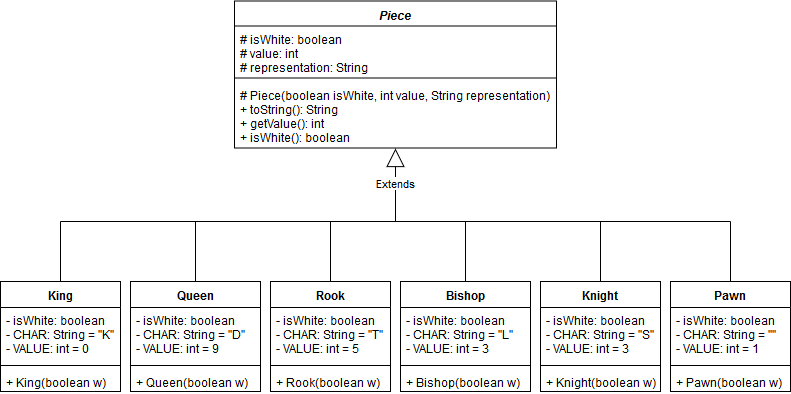
\includegraphics[width=1\linewidth]{Diagramme/Pieces}
		\captionof{figure}{Pieces}
		\label{fig:pieces}
		\end{minipage}
		\begin{itemize}
			\item \textbf{\textit{Piece}}
			
				Stellt das abstrakte Konzept einer Schachfigur dar.
				
				Attribute
				\newline
				\rule{\textwidth}{1pt}
				\begin{description}			
					\item \textbf{\textit{isWhite:}} Speichert, ob die Figur weiß ist.
					\item \textbf{\textit{value:}} Speichert den Wert einer Figur ab.
					\item \textbf{\textit{representation:}} Speichert das repräsentative Zeichen einer Figur ab.
				\end{description}
				Methoden
				\newline
				\rule{\textwidth}{1pt}
				\begin{description}
					\item \textbf{\textit{Piece(isWhite: boolean, value: int, representation: String:}} Erzeugt eine neue Figur, setzt alle Attribute auf die jeweiligen übergebenen Werte.
					\item \textbf{\textit{toString():}} Gibt \textbf{\textit{representation}} zurück.
					\item \textbf{\textit{getValue():}} Gibt \textbf{\textit{value}} zurück.
					\item \textbf{\textit{isWhite():}} Gibt \textbf{\textit{isWhite}} zurück.				
				\end{description}
			
			\item \textbf{\textit{King}}
				Stellt einen König dar.
				
				Attribute
				\newline
				\rule{\textwidth}{1pt}
				\begin{description}			
					\item \textbf{\textit{CHAR:}} Die Repräsentation eines Königs, wird auf K gesetzt.
					\item \textbf{\textit{VALUE:}} Der Wert eines Königs, wird auf 0 gesetzt, da dem König an sich kein Wert zugewiesen werden kann.
				\end{description}
				Methoden
				\newline
				\rule{\textwidth}{1pt}
				\begin{description}
					\item \textbf{\textit{King(w: boolean):}} Erzeugt einen neuen König. Dazu wird der Konstruktor von \textbf{\textit{Piece}} aufgerufen, als Parameter werden w, \textbf{\textit{VALUE}}, und \textbf{\textit{CHAR}} übergeben.
					\item \textbf{\textit{getMovement(Position p, BoardState b):}} Gibt eine Liste der Züge zurück, die ein König auf dem gegebenen Schachbrett von der gegebenen Position aus ausführen kann, inklusive Rochade. Dabei wird nicht berücksichtigt, ob sich der König nach dem Zug in Schach befinden würde.
				\end{description}
				
			
			\item \textbf{\textit{Queen}}
			
				Stellt eine Dame dar.
				
				Attribute
				\newline
				\rule{\textwidth}{1pt}
				\begin{description}				
					\item \textbf{\textit{CHAR:}} Die Repräsentation einer Dame, wird auf D gesetzt.
					\item \textbf{\textit{VALUE:}} Der Wert einer Dame, wird auf 9 gesetzt.
				\end{description}
				Methoden
				\newline
				\rule{\textwidth}{1pt}
				\begin{description}	
					\item \textbf{\textit{Queen(w: boolean):}} Erzeugt eine neue Dame. Dazu wird der Konstruktor von \textbf{\textit{Piece}} aufgerufen, als Parameter werden w, \textbf{\textit{VALUE}}, und \textbf{\textit{CHAR}} übergeben.
					\item \textbf{\textit{getMovement(Position p, BoardState b):}} Gibt eine Liste der Züge zurück, die eine Dame auf dem gegebenen Schachbrett von der gegebenen Position aus ausführen kann. Dabei wird nicht berücksichtigt, ob sich der König des ziehenden Spielers nach dem Zug in Schach befinden würde.
				\end{description}
			
			\item \textbf{\textit{Rook}}
				
				Stellt einen Turm dar.
				
				Attribute
				\newline
				\rule{\textwidth}{1pt}
				\begin{description}
					\item \textbf{\textit{CHAR:}} Die Repräsentation eines Turms, wird auf T gesetzt.
					\item \textbf{\textit{VALUE:}} Der Wert eines Turms, wird auf 5 gesetzt.
				\end{description}
				Methoden
				\newline
				\rule{\textwidth}{1pt}
				\begin{description}	
					\item \textbf{\textit{Rook(w: boolean):}} Erzeugt einen neuen Turm. Dazu wird der Konstruktor von \textbf{\textit{Piece}} aufgerufen, als Parameter werden w, \textbf{\textit{VALUE}}, und \textbf{\textit{CHAR}} übergeben.
					\item \textbf{\textit{getMovement(Position p, BoardState b):}} Gibt eine Liste der Züge zurück, die ein Turm auf dem gegebenen Schachbrett von der gegebenen Position aus ausführen kann. Dabei wird nicht berücksichtigt, ob sich der König des ziehenden Spielers nach dem Zug in Schach befinden würde.
				\end{description}
			
			\item \textbf{\textit{Bishop}}
				
				Stellt einen Läufer dar.
				
				Attribute
				\newline
				\rule{\textwidth}{1pt}
				\begin{description}			
					\item \textbf{\textit{CHAR:}} Die Repräsentation eines Läufers, wird auf L gesetzt.
					\item \textbf{\textit{VALUE:}} Der Wert eines Läufers, wird auf 3 gesetzt.
				\end{description}
				Methoden
				\newline
				\rule{\textwidth}{1pt}	
				\begin{description}				
					\item \textbf{\textit{Bishop(w: boolean):}} Erzeugt einen neuen Läufer. Dazu wird der Konstruktor von \textbf{\textit{Piece}} aufgerufen, als Parameter werden w, \textbf{\textit{VALUE}}, und \textbf{\textit{CHAR}} übergeben.
					\item \textbf{\textit{getMovement(Position p, BoardState b):}} Gibt eine Liste der Züge zurück, die ein Läufer auf dem gegebenen Schachbrett von der gegebenen Position aus ausführen kann. Dabei wird nicht berücksichtigt, ob sich der König des ziehenden Spielers nach dem Zug in Schach befinden würde.
				\end{description}
			
			\item \textbf{\textit{Knight}}
				
				Stellt einen Springer dar.
				
				Attribute
				\newline
				\rule{\textwidth}{1pt}
				
				\begin{description}			
					\item \textbf{\textit{CHAR:}} Die Repräsentation eines Springers, wird auf S gesetzt.
					\item \textbf{\textit{VALUE:}} Der Wert eines Springers, wird auf 3 gesetzt.
				\end{description}
				Methoden
				\newline
				\rule{\textwidth}{1pt}
				\begin{description}
					\item \textbf{\textit{Knight(w: boolean):}} Erzeugt einen neuen Springer. Dazu wird der Konstruktor von \textbf{\textit{Piece}} aufgerufen, als Parameter werden w, \textbf{\textit{VALUE}}, und \textbf{\textit{CHAR}} übergeben.
					\item \textbf{\textit{getMovement(Position p, BoardState b):}} Gibt eine Liste der Züge zurück, die ein Springer auf dem gegebenen Schachbrett von der gegebenen Position aus ausführen kann. Dabei wird nicht berücksichtigt, ob sich der König des ziehenden Spielers nach dem Zug in Schach befinden würde.
				\end{description}
			
			\item \textbf{\textit{Pawn}}
				
				Stellt einen Bauern dar.
				
				Attribute
				\newline
				\rule{\textwidth}{1pt}
				
				\begin{description}				
					\item \textbf{\textit{CHAR:}} Die Repräsentation eines Bauerns, wird auf B gesetzt.
					\item \textbf{\textit{VALUE:}} Der Wert eines Bauerns, wird auf 1 gesetzt.
				\end{description}
				Methoden
				\newline
				\rule{\textwidth}{1pt}
				\begin{description}
					\item \textbf{\textit{Pawn(w: boolean):}} Erzeugt einen neuen Bauern. Dazu wird der Konstruktor von \textbf{\textit{Piece}} aufgerufen, als Parameter werden w, \textbf{\textit{VALUE}}, und \textbf{\textit{CHAR}} übergeben.
					\item \textbf{\textit{getMovement(Position p, BoardState b):}} Gibt eine Liste der Züge zurück, die ein Bauer auf dem gegebenen Schachbrett von der gegebenen Position aus ausführen kann, inklusive en passant, Doppelsprung und Umwandlung. Dabei wird nicht berücksichtigt, ob sich der König des ziehenden Spielers nach dem Zug in Schach befinden würde.
				\end{description}
		\end{itemize}		
		\newpage		
		
		\subsection{GUI}
		\subsubsection{Activities}
		\begin{minipage}{\linewidth}
			\centering
			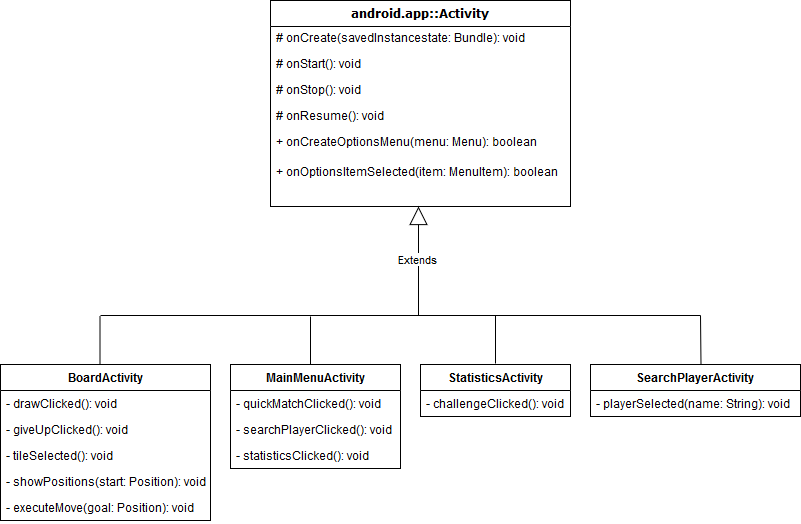
\includegraphics[width=1\linewidth]{Diagramme/ActivityDiagram}
			\captionof{figure}{Activities}
			\label{fig:activities}
		\end{minipage}
	
		\subsubsection{Dialoge}
		\begin{minipage}{\linewidth}
			\centering
			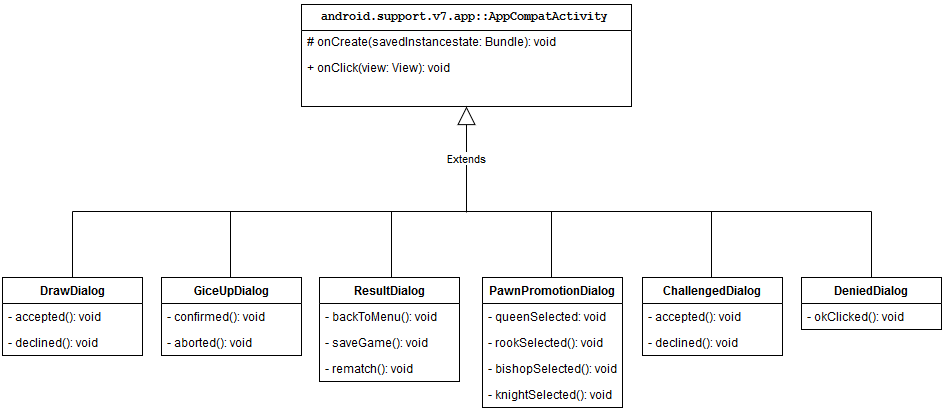
\includegraphics[width=1\linewidth]{Diagramme/DialogDiagram}
			\captionof{figure}{Dialoge}
			\label{fig:dialoge}
		\end{minipage}
		\newpage
		\subsection{Server}
		\begin{minipage}{\linewidth}
			\centering
			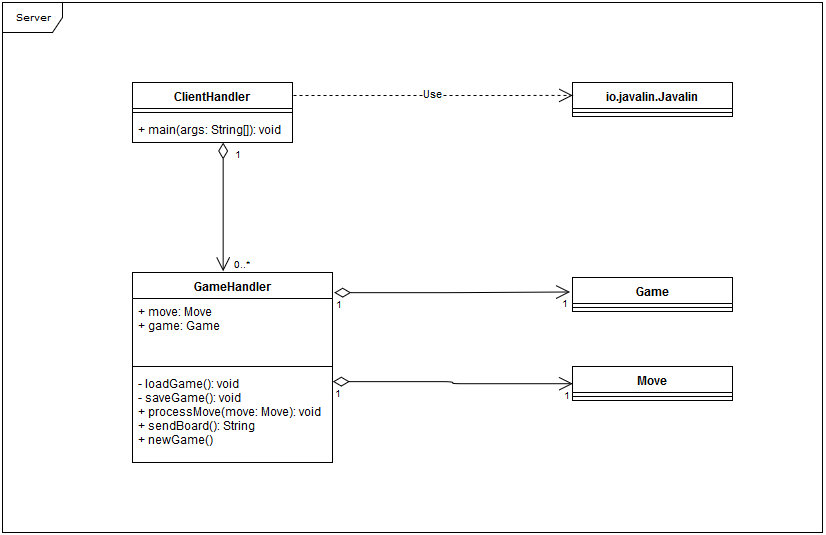
\includegraphics[width=1\linewidth]{Diagramme/Server}
			\captionof{figure}{Server}
			\label{fig:server}
		\end{minipage}
		\begin{itemize}
			\item \textbf{ClientHandler}
			
			Verwaltet eingehende Anfragen an den Server.
			
			Methoden
			\newline
			\rule{\textwidth}{1pt}
			\begin{description}
				\item \textbf{\textit{main(String[] args):}}
				Die main Methode des Servers. Hier wird der Javalin Server gestartet. Je nach Anfrage wird ein GameCreator, ein BoardHandler oder ein MoveHandler erstellt. 
			\end{description} 
	
	
			\item \textbf{GameCreator}
			
				Attribute
				\newline
				\rule{\textwidth}{1pt}
				\begin{description}
					\item \textbf{\textit{player1: String:}}
					Spieler 1 des neuen Spiels.
					\item \textbf{\textit{player2: String:}}
					Spieler 2 des neuen Spiels.
				\end{description}	
				Methoden
				\newline
				\rule{\textwidth}{1pt}
				\begin{description}
					\item \textbf{\textit{create(player1: String, player2: String):}}
					Erstellt einen neuen Spiel-Eintrag in der Datenbank. Benutzt dazu einen DatabaseHandler.
				\end{description}
		
		
			\item \textbf{BoardHandler}
			
				Attribute
				\newline
				\rule{\textwidth}{1pt}
				\begin{description}
					\item \textbf{\textit{board: BoardState}}
					Aktueller Zustand des Bretts.
				\end{description}	
				Methoden
				\newline
				\rule{\textwidth}{1pt}	
				\begin{description}
					\item \textbf{\textit{getBoard(player: String): String}}
					Lädt das entsprechende Spielbrett aus der Datenbank. Verwendet ebenfalls einen DatabaseHandler.
				\end{description}
		
		
			\item \textbf{MoveHandler}
				
				Attribute
				\newline
				\rule{\textwidth}{1pt}
				\begin{description}
					\item \textbf{\textit{move: Move}}
					Der Zug der überprüft und ausgeführt wird.
					\item \textbf{\textit{board: BoardState}}
					Das Spielbrett auf dem dieser Zug ausgeführt werden soll.
				\end{description}
				Methoden
				\newline
				\rule{\textwidth}{1pt}	
				\begin{description}
					\item \textbf{\textit{processMove(move: Move): BoardState}}
					Laden und Speichern erfolgen wieder über einen DatabaseHandler.
					Überprüft ob die Kombination aus Brett und Zug gültig ist. Wendet den Zug an, falls dieser gütlig ist.
					Speichert das neue Brett ab und benachrichtigt anschließend den Gegner.
				\end{description}
		
		
			\item \textbf{DatabaseHandler}
			
				Legt die Methoden fest, die ein DatabaseHandler implementieren muss.
				
				Methoden
				\newline
				\rule{\textwidth}{1pt}
				\begin{description}
					\item \textbf{\textit{newEntry(player1: String, player2: String):void}}	
					Soll einen neuen Datenbankeintrag mit Spieler 1 , Spieler 2 und einem neuen Brett anlegen.
					\item \textbf{\textit{loadGame(player: String): String}}
					Soll das zum Spieler zugehörige Brett aus der Datenbank laden.
					\item \textbf{\textit{saveGame(player: String): void}}
					Soll ein Brett wieder in die Datenbank speichern.
				\end{description}
			
		
			\item \textbf{FirebaseHandler}
			
				Verwaltet die Verbindung zur Firebase Datenbank.
				
				Methoden
				\newline
				\rule{\textwidth}{1pt}
				\begin{description}
					\item \textbf{\textit{newEntry(player1: String, player2: String):void}}	
					Erstellt einen neuen Eintrag mit beiden Spielern und einem neuen Brett.
					\item \textbf{\textit{loadGame(player: String): String}}
					Lädt das zum Spieler zugehörige Brett aus der Datenbank.
					\item \textbf{\textit{saveGame(player: String): void}}
					Speichert das Brett wieder ab.
				\end{description}
			
			
		\end{itemize}
	\section{Sequenzdiagramm}
\end{document}